\documentclass[14pt, a4paper]{extarticle}
% Русская локализация
\usepackage[english,russian]{babel}


\usepackage{appendix}
\usepackage{alphabeta}

% Использование математических шрифтов
\usepackage{unicode-math}

% Шрифты
\usepackage{fontspec}
\usepackage{courier}
\defaultfontfeatures{Ligatures={TeX},Renderer=Basic}
\setmainfont[Ligatures={TeX}]{Times New Roman}
\setmonofont{Courier New}
\setmathfont{XITS Math}

% Расширенные ссылки
\usepackage{nameref}

% Оформление URL
\usepackage{xurl}
\usepackage{hyperref}
\hypersetup{
  colorlinks,
  citecolor=black,
  filecolor=black,
  linkcolor=black,
  urlcolor=black,
  breaklinks=true,
}
\urlstyle{same}

% Поддержка изображений
\usepackage{graphicx}
\graphicspath{{./images/}}
\DeclareGraphicsExtensions{.jpg,.png}
\usepackage{svg}

% Таблицы
\usepackage{tabularx}
\usepackage{tabulary}
\usepackage{ltablex}
\usepackage{multirow}
\usepackage{hhline}
% Выравнивание по левому краю, с многострочностью
\newcolumntype{s}{>{\raggedright\arraybackslash}X}

% Поддержка листингов
\usepackage{listings}
\lstdefinestyle{gost}{
  basicstyle=\ttfamily\footnotesize,
  breakatwhitespace=false,
  breaklines=true,
  keepspaces=true,
  showspaces=false,
  showstringspaces=false,
  frame=single
}
\lstset{style=gost}%

% Отступ первой строки первого абзаца
\usepackage{indentfirst}
\linespread{1.25}

% Размер полей в документе
\usepackage{geometry}
\geometry{left=3cm}
\geometry{right=1cm}
\geometry{top=2cm}
\geometry{bottom=2cm}

% Абзацный отступ
\setlength{\parindent}{1.25cm}

% Отступ для элементов в списке
\usepackage{enumitem}
\setlist{left=\parindent, labelsep=1cm, itemsep=0pt, topsep=0pt}

% Загрузка pdf-документов (нужно для титульных листов)
\usepackage[final]{pdfpages}
% Возможность поворота pdf файло
\usepackage{pdflscape}
\usepackage{everypage}

\newcommand{\Lpagenumber}{\ifdim\textwidth=\linewidth\else\bgroup%
    \dimendef\margin=0 %use \margin instead of \dimen0
    \ifodd\value{page}\margin=\oddsidemargin
    \else\margin=\evensidemargin%
    \fi

\raisebox{\dimexpr-\topmargin-\headheight-\headsep-0.5\linewidth}[0pt][0pt]{%
      \rlap{\hspace{\dimexpr-\margin+\textheight+\footskip}%
        \llap{\rotatebox{90}{\thepage}}}}%
    \egroup\fi}
\AddEverypageHook{\Lpagenumber}%

\usepackage{float}
% Форматирование подписей
\usepackage{caption}

\usepackage{newfloat}
% \DeclareCaptionType{listing}

\DeclareCaptionLabelSeparator{emdash}{\;\textemdash\;}
\captionsetup[figure]{name={Рисунок}, labelsep=emdash, justification=centering,
position=above, singlelinecheck=off, font={small, bf}, labelfont=bf, skip=6pt}
\captionsetup[table]{name={Таблица}, labelsep=emdash,
justification=raggedright, position=top, singlelinecheck=off, font={small, it},
labelfont=it, skip=6pt, margin=0cm}
% \captionsetup[lstlisting]{labelsep=emdash, justification=raggedright,
% position=top, singlelinecheck=off, font={small, it}, labelfont=it, skip=6pt,
% margin=0cm}

% Нумеровать внутри заголовков первого уровня
\counterwithin{figure}{section}
\counterwithin{table}{section}
% \counterwithin{lstlisting}{section}
\AtBeginDocument{\counterwithin{lstlisting}{section}}

% Отключение переносов текста
\usepackage{ragged2e}
\justifying
\tolerance=500
\hyphenpenalty=10000
\emergencystretch=3em

% Форматирование заголовков
\usepackage{titlesec}
% Оформление заголовка первого уровня
% Полужирное начертание
% Кегль 18 пт
% С новой страницы
\titleformat{\section}[block]
{\newpage\bfseries\fontsize{18pt}{21.6pt}\selectfont}
{\thesection}
{1em}{}
% Оформление ненумерованных заголовков (Введение, Содержание, список
% источников, и.т.д.)
\titleformat{name=\section,numberless}[block]
{\centering\newpage\bfseries\fontsize{18pt}{21.6pt}\selectfont}
{}
{0em}{}{}
% Отступы у заголовков первого уровня
\titlespacing{\section}
{\parindent}% отступ слева (равен 1.25 см, как у отступа первой строки абзаца)
{0em}% интервал перед
{10mm}% интервал после
% Оформление заголовков второго уровня
\titleformat{\subsection}[block]
{\bfseries\fontsize{16pt}{19.2pt}\selectfont}
{\thesubsection}
{1em}{}
% Отступы у заголовков второго уровня
\titlespacing{\subsection}
{\parindent}% пробел слева
{15mm}% отступ перед
{10mm}% отступ после
% Оформление заголовков второго уровня
\titleformat{\subsubsection}[block]
{\bfseries\selectfont}
{\thesubsection}
{1em}{}
% Отступы у заголовков второго уровня
\titlespacing{\subsubsection}
{\parindent}% пробел слева
{15mm}% отступ перед
{10mm}% отступ после


% Оформление заголовков в содержании
\usepackage{titletoc}
\contentsmargin{0pt}
\renewcommand\contentspage{\thecontentspage}
\dottedcontents{section}[2.3em]{}{2.3em}{5pt}
\dottedcontents{subsection}[2.3em]{}{2.3em}{5pt}
% Оформление приложений
\usepackage{appendix}
\renewcommand\appendixpagename{ПРИЛОЖЕНИЯ}

% Подключение biblatex, с использованием стиля gost-numeric
\usepackage[
citestyle=gost-numeric,
style=gost-numeric,
blockpunct=emdash,
backend=biber,
sorting=none
]{biblatex}
% Запрет разрыва url ссылок
\defcounter{biburlnumpenalty}{3000}
\defcounter{biburlucpenalty}{6000}
\defcounter{biburllcpenalty}{9000}
% Добавление полей для ссылок и даты обращения к ним
\DeclareFieldFormat{url}{Режим доступа: #1}
\DeclareFieldFormat{urldate}{(Дата обращения: #1)}
\renewcommand*{\entrysetpunct}{\par\nopunct\!\!}
% Использовать prac.bib как источник
\addbibresource{diploma.bib}
% Форматирование заголовка библиографии
\defbibheading{bibliography}[\bibname]{%
  \section*{\centering #1}%
  \markboth{#1}{#1}}
  
\usepackage{etoolbox}
\AtBeginEnvironment{tabularx}{\fontsize{12pt}{14pt}\selectfont}


\usepackage{lipsum}
\usepackage{csquotes}

\begin{document}
\def\contentsname{СОДЕРЖАНИЕ}

% Загрузка титула
% \pagenumbering{gobble}
% \begin{titlepage}
%   
\includepdf{title}
%   
\includepdf[pages={1-5}]{title}
% \end{titlepage}
% \pagenumbering{arabic}
% \setcounter{page}{7}

\setcounter{page}{1}
% Содержание
\tableofcontents

\section*{ВВЕДЕНИЕ}
\phantomsection
\addcontentsline{toc}{section}{ВВЕДЕНИЕ}

Исследуемым объектом в рамках проекта является сервис хранения и обработки
данных модуля потребительского кредитования. Этот модуль включает в
себя ответственность за управление ипотечными и кредитными продуктами, так же
за хранение и обработку данных клиентов и генерацию отчетов, как по клиентам
так и работе модуля.

Актуальность темы исследования обусловлена стремительным развитием информационных
технологий и их внедрением во все сферы социально-экономической жизни, включая сектор
финансовых технологий. Кредитные организации в настоящее время находятся в условиях 
сильной конкуренции, а это вынуждает активно внедрять новые технологии, в частности 
цифровые технологии, которые позволяют оптимизировать затраты и внутренние процессы, 
повышать качество обслуживания клиентов и обеспечивать устойчивость бизнес-моделеи.
В этом ключе важное значение приобретает проектирование и фунциольное моделирование
ИТ-инфраструктуры одного из ключевых элементов, который обеспечивает эффективаность
функционирования автоматизированных кредитных систем, а именно модуля потребительского 
кредитования.

В отечественной и зарубежной литературе существует много работ, рассматриващих
проблемы проектирования и моделирования ИТ-инфраструктуры в которых так же 
рассматриваются архитектурные подходы, выбор технических решений и методы оптимизации 
процессов. Однако в условиях быстро меняющейся регулятороной и потребительской среды 
задача создания адаптированной, масштабируемой и безопасной ИТ-инфраструктуры с учетом 
специфики бизнес-процессов конкретной организации остается актуальной.

Целью данной работы является проектирование и функциональное моделирование
ИТ-инфраструктуры, поддерживающей модуль потребительского кредитования в 
кредитной организации, включающего описание архитектуры и обоснование выбранного
программно-аппаратного решения.

Для достижения поставленной цели в работе решаются следующие задачи:

\begin{enumerate}
  \item Анализ вариантов поставки информационно-технологического сервиса;
  \item Анализ вариантов компонентов ИТ-инфраструктуры и обоснование выбранного варианта;
  \item Выбор системного программного обеспечения;
  \item Моделирование топологии развертывания;
  \item Составление спецификации рабочих станций;
  \item Моделирование топологии развертывания инструментального программного обеспечения;
  \item Анализ сетевой инфраструктуры и моделирование сетевой топологии.
\end{enumerate}

Практическая значимость работы заключается в возможности использования представленных
разработок для модернизации или внедрения модулей автоматизированных систем 
потребительского кредитования в ИТ-инфраструктуру кредитных организаций, что 
способствует повышению надежности, безопасности, отказаустойчивости и производительности.

\section*{ГЛОССАРИЙ}
\phantomsection
\addcontentsline{toc}{section}{ГЛОССАРИЙ}
\begin{raggedright}
  VPC --- Virtual Private Cloud (виртуальная частная сеть). \\
  ЦОД --- Центр обработки данных. \\
  СХД --- Система хранения данных. \\
  FC --- Fiber Channel (оптоволоконный канал). \\
  ИТ --- Информационные технологии. \\
  ИТ-инфраструктура --- Информационно-технологическая инфраструктура. \\
  UML --- Unified Modeling Language (Унифицированный язык моделирования) \\
\end{raggedright}

\section{ПРОИЗВОДСТВЕННАЯ ПРАКТИКА}

\subsection{Анализ вариатнов поставки информационно-технологического сервиса}

В работе произведен анализ четырех вариантов поставки
информационно-технологического сервиса, который включает в себя выбор между
такими вариантами поставки, как полностью самостоятельный, облачный (SaaS, Paas, IaaS),
мульти-облачный и гибридный. На основе анализа выбран, как самый оптимальный вариант
поставки, гибридный вариант, который включает в себя как облачные решения, так и
самостоятельные решения.

Полностью облачный сервис \cite{micrasoft-azure-book} по одному из моделей SaaS,
PaaS или IaaS, позволяет снизить затраты на создержание и поддержку ИТ-инфраструктуры,
но не является лучшим решением, так как вводит за собой ряд ограничений, таких как
сильная зависимость от поставщика, ограниченные возможности кастомизации и настройки,
а также, что является критичным, возможные проблемы с безопасностью и сохранностью данных.

Мульти-облачный вариант, подразумевает под собой так же использование облачной
инфраструктуры, но в отличие от полностью облачного варианта, позволяет использовать
разные облачные решения от разных поставщиков, что позволяет избежать
некоторых проблем, связанных с безопасностью и кастомизацией. Однако, данный
вариант так же не является оптимальным, так как требует высококвалифицированных
специалистов для поддержки и настройки, а так же имеет риски конфликтов совместимости,
что существенно сказывается на затратах.

Полностью самостоятельный вариант поставки заключается в создании и поддержке
ИТ-инфраструктуры на базе собственных ресурсов. Данный подход избавляет от
каких-либо зависимостей от поставщиков облачных ресурсов и позоляет полностью
контролировать все аспекты инфраструктры, однако требует значительныз затрат и
больших вложений, кроме того такой вариант сложен в поддержке и сложно масштабируем
в отличие от облачных решений.

Гибридный подход позволяет совместное исопльзование облачных решений и собственных
ресурсов. Такой вариант позволяет гибко масштабировать инфраструктуру на облачных
решениях и использовать собственные ресурсы для таких критически важных задач, как
хранение и обработка персональных данных используемых в модуле потребительского
кредитования требующего соблюдения требований безопасности и защиты персональных
данных. Хранение данных на собственных ресурсах позволяет избежать проблем с
безопасностью и изначально запланировать архитектуру хранения данных с учетом
требований регуляторов и Федерального закона №152-ФЗ <<О персональных данных>>.

Поставщик облачных услуг - это отечественная компания <<Yandex Cloud>> \cite{yandex-cloud-for-finance}.
<<Yandex Cloud>>, как облачный провайдер и платаформа присутствует в реестре Минцифры
и поддерживает экосистему отечественного программного обеспечения и сервисов. Платформа
предоставляет широкий спектр услуг, включая облачные вычисления, хранение данных, базы данных.
Даграама \ref{fig:ya-clound-hybrid-conneciton-diagram} иллюстрирует гибридную архитектуру,
которая может быть применена при интеграции собственной инфраструктры в ЦОДе с приватным
облаком (VPC) <<Yandex Cloud>>. На диаграмме отображено, что подключение к ЦОД в точке
присутствия можно осуществить через собственный канал связи или канал связи сетевого
оператора. Так как решение использовать собственные каналы связи является дорогим и
неоправданным, то использование варианта подключения через канал связи сетевого оператора
ялвяется лушим решением до значительного роста нагрузки.

\begin{figure}[H]
  \centering
  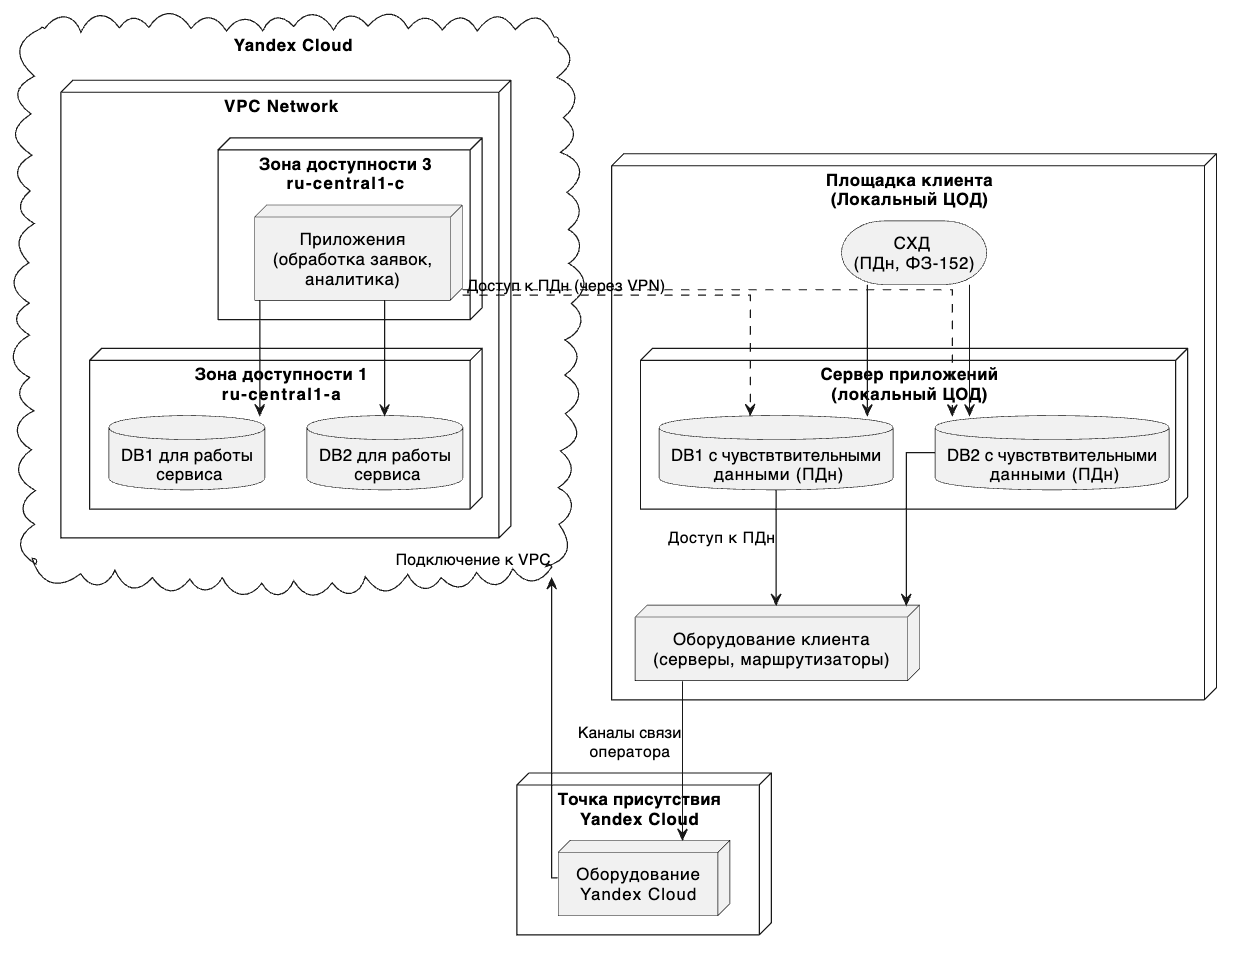
\includegraphics[width=0.62\textwidth]{ya-clound-hybrid-conneciton-diagram.png}
  \caption{UML Диаграмма интеграции гибридного решения с <<Yandex Cloud>>}
  \label{fig:ya-clound-hybrid-conneciton-diagram}
\end{figure}

\subsection{Анализ вариантов компонентов ИТ-инфраструктуры}

В данном разделе произведен анализ возможных компонентов ИТ-инфраструктуры,
которые могут быть использованы в проектируемой инфраструктуре. Основными
компонентами являются серверы, системы хранения данных, сетевое оборудование,
системы резервного копирования и восстановления, системы виртуализации и облачные решения.

Собственный ЦОД будет использоваться исключительно для хранения и обработки чувствительных 
данных, а все  вычисления будут производиться в облаке. Это позволит снизить затраты на
содержание и поддержку большой ИТ-инфраструктуры, где надо озаботиться мощными
серверами для обработки и поддержания данных приложений и сервисов. Хранение 
данных и обработка в собственном ЦОДе позволит избежать проблем с безопасностью и защитой
персональных данных, так как все данные будут храниться на собственных серверах,
которые будут находиться под контролем и защитой самой кредитной организации.

Инфраструктура включает в себя такие компоненты, как два сервера, два коммутатора 
и два маршрутизатора и не включает в себя отдельные СХД. Это оправдано использованием
серверов с поддержкой NVMe и SSD дисков, которые обеспечивают высокую скорость
чтения и записи данных, что позволяет использовать их в качестве аппааратных СХД
в всязке с протоколом <<ISCSI>>. <<ProxMox>> на серверах позволяет 
на дополнительном уровне обеспечивать отказаустойчивость и защиту данных.

В качестве сервера выбрана модель <<Гравитон>> С2122ИУ \cite{graviton-server-s2121iv} 2U.
Выбранный сервер поддерживает до двух процессоров Intel Xeon 4-го поколения, имеет 
большой потенциал для увеличения объема оперативной памяти, обеспечивает надежность
благодаря резервному блоку питания, официально поддерживает российские ОС (Astra Linux,
BaseALT, Red OS и др.), что соответствует требованиям регуляторов и имеет физическую
компоновку в 2U, что упрощает инсталяцию и обслуживание. Важная особенность данного
сервера заключается в поддержке до 12 NVMe и SATA дисков, c поддержкой быстрой замены. 
Это позволяет иметь достаточный объем памяти и производительности для обработки
данных и использования в качестве СХД. Так как сервера два, то они связаны между собой
в кластер с использованием программного обеспечения <<ProxMox>> \cite{prox-mox}, а 
децентрализованное хранение данных производится с использованием <<ISCSI>> \cite{iscsi}.

Сетевая инфраструктура состот из двух маршрутизаторов и двух коммутаторов, где каждый 
из коммутаторов связан c обоими маршрутизаторами. Это позволяет обеспечить отказаустойчивость
как на уровне устройств, так и на уровне каналов связи. Маршрутизатор выбран от производителя 
<<Элтех>> ESR-3100 \cite{eltech-ESR-3100} 1U. Он имеет 8 портов 1G и 8 портов 10G, 
что позволяет обеспечить  высокую скорость передачи данных и два сменных блока питания. 
Количество портов позволяет для всех существующих соединений использовать 10G порты, а так
же оставить пространство для будущего маштабирования. Коммутатор выбран от этого же 
производителя и имеет код MES2300-24 \cite{eltech-MES2300-24} L3. Пропуская способность 
коммутатора составляет 128 Гбит/с, что позволяет обеспечить высокую скорость передачи данных
и поддерживает до 24 портов 1G и 4 порта 10G, что тоже оставляет простарнство под будущее
масштабирование с ростом количества данных и узлов.

Так как маршрутризатора 2, то каждый из них имеет своего провайдера связи для 
снижения вероятность отказа. В качестве провайдеров связи выбраны компании <<Ростелеком>> 
\cite{rostelekom} и <<МТС>> \cite{mts}. Это позволит 
обеспечить высокую скорость передачи данных и надежность связи. Благоря каналам 
связей провайдеров  становится доступной возможность передачи данных до точки присутствия 
<<Yandex Cloud>>, после чего трафик направлется в облако.

Инфраструктура внутри облака <<Yandex Cloud>> состоит из VPC в котором арендуются 
нужные ресурсы. VPC включает в себя виртуальную машину на 20 CPU ядер и 60 ГБ оперативной
памяти, объем памяти виртуальной машины состовляет 1 ТБ с показателями IOPS 20000/32000 и
до 450 Мб/с. (110к) В облачную инфраструктуру так же входит управляемый кластер <<K8S>>
\cite{k8s} с 3 узлами, 2 ТБ памяти и 60 CPU ядер и 180 ГБ оперативной памяти (388к). На кластере 
<<K8S>> развернуты все приложения и сервисы, которые обеспечивают работу модуля
потребительского кредитования. Базы данных <<PostgreSQL >> \cite{postgresql} и 
<<MongoDB>> \cite{mongodb} так же являются управляемыми и входят в базоый пакет
<<Yandex Cloud>>. Топология развертывания гибирдной инфраструктуры с указанием 
компонентов представлена на диаграмме \ref{fig:components-structure}.

\begin{figure}[H]
  \centering
  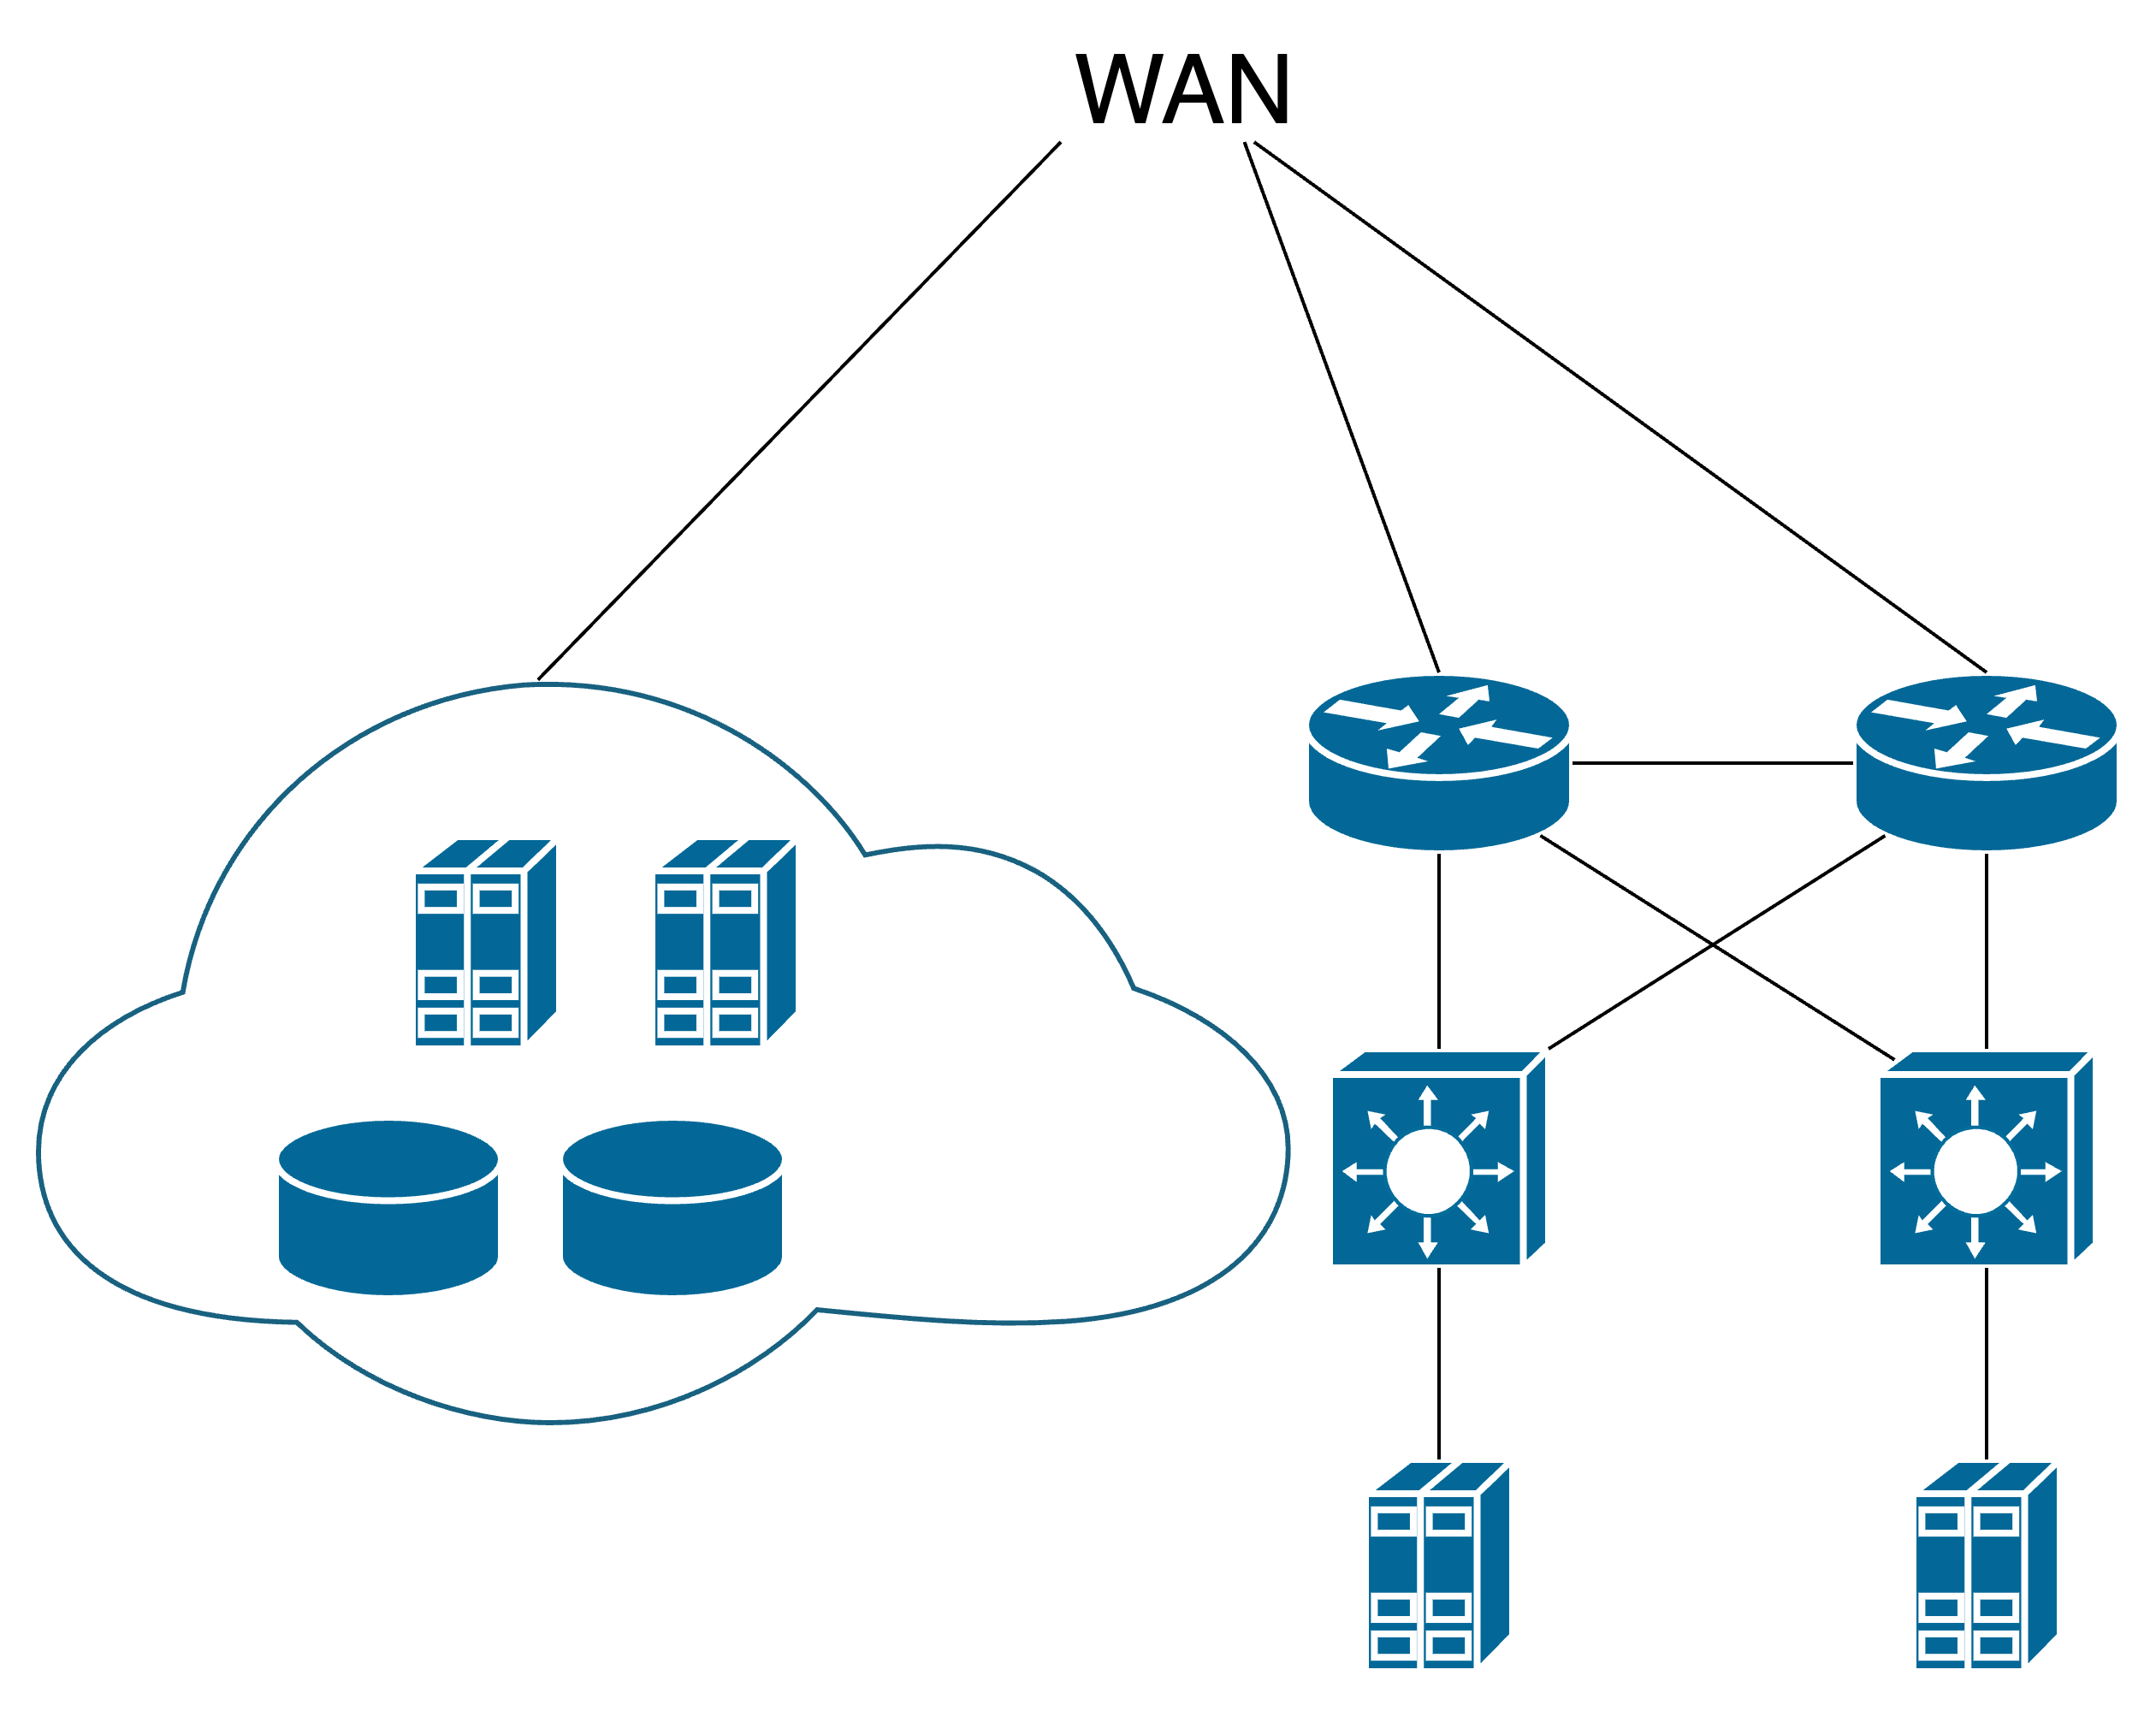
\includegraphics[width=1\textwidth]{components-structure.png}
  \caption{Диаграмма развертывания гибридной инфраструктуры}
  \label{fig:components-structure}
\end{figure}


\section{Заключение}


% used resources list
\begingroup
\let\itshape\upshape
\sloppy
\raggedright
\printbibliography[title=СПИСОК ИСПОЛЬЗУЕМЫХ ИСТОЧНИКОВ]
\phantomsection
\addcontentsline{toc}{section}{СПИСОК ИСПОЛЬЗУЕМЫХ ИСТОЧНИКОВ}
\endgroup
% used resources list

\end{document}